%% LyX 2.0.3 created this file.  For more info, see http://www.lyx.org/.
%% Do not edit unless you really know what you are doing.
\documentclass[english,ngerman]{article}
\usepackage[T1]{fontenc}
\usepackage[latin9]{inputenc}
\usepackage{amsmath}
\usepackage{graphicx}
\usepackage{babel}
\begin{document}

\title{Lines for OpenGlider}

\maketitle

\section{line-sag:}


\subsection{dgl:}

\begin{center}
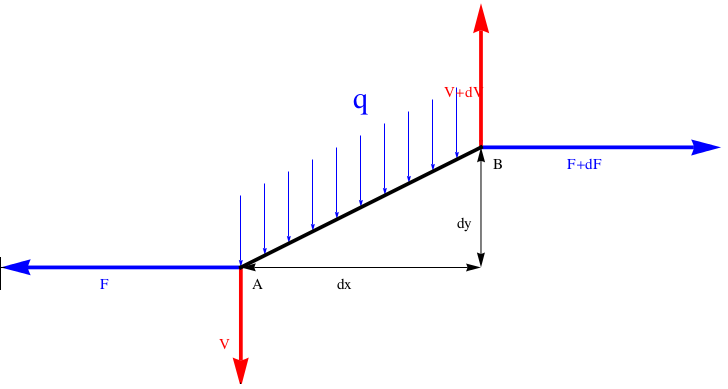
\includegraphics[scale=0.2]{pictures/deifferential}
\par\end{center}

\begin{align*}
\sum F_{x}=0=V+dV-V-q\cdot dx\Rightarrow dV=q\cdot dx\Rightarrow\frac{dV}{dx}=V'=-q\\
\sum F_{y}=0=F+dF-F\Rightarrow dF=0\Rightarrow F'=0\\
\frac{dy}{dx}=y'(x)=\frac{V(x)}{F(x)}\Rightarrow y''(x)=\frac{V'(x)}{F(x)}-\frac{V(x)\cdot F'(x)}{F(x)^{2}}=\frac{V'(x)}{F}=-\frac{q}{F}\\
y''(x)=-\frac{q}{F}
\end{align*}



\subsection{projection}

\begin{center}
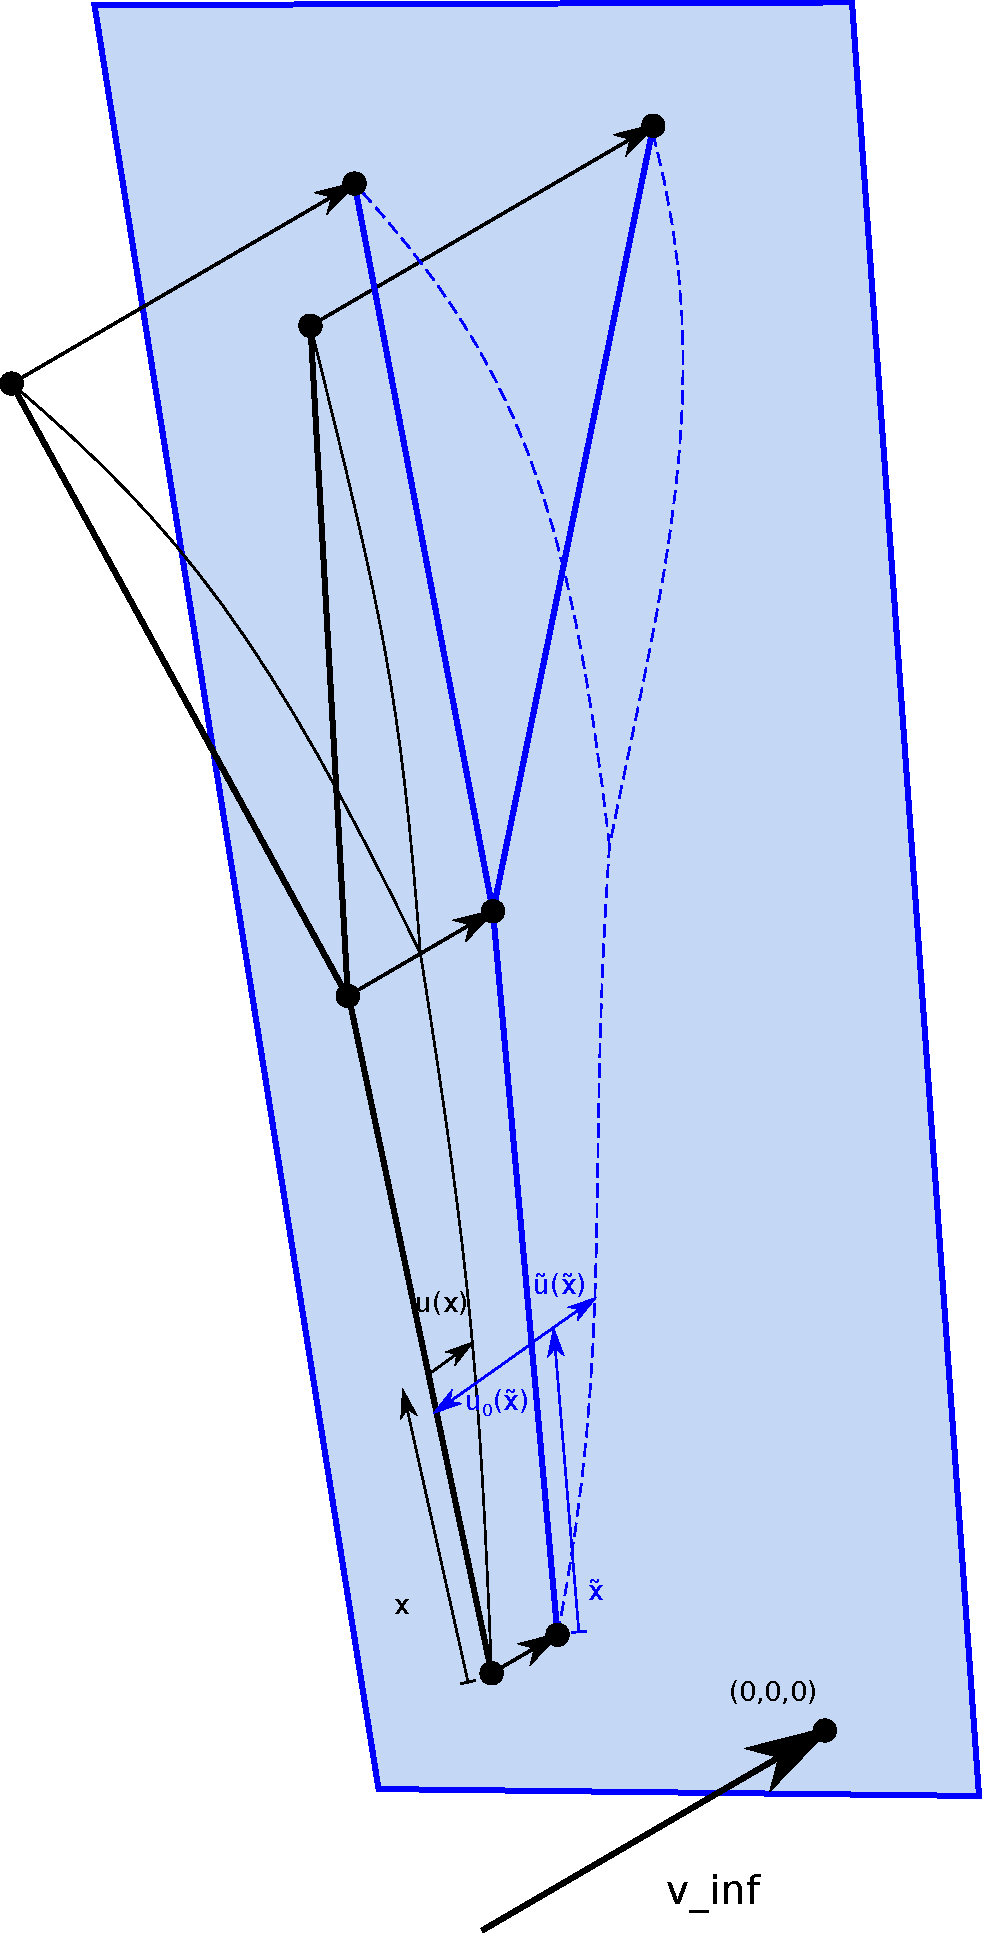
\includegraphics[scale=0.3]{pictures/sag}
\par\end{center}

\begin{align*}
u(x)=y(x)\quad u''(x)=-\frac{q}{F}\\
u(x)=\tilde{u}(x)+u_{0}(x)\\
u'(x)=\tilde{u}'(x)+u'_{0}\\
u''(x)=\tilde{u}''(x)=-\frac{q}{F}\\
\\
\tilde{u}''(x)=-\frac{q}{F}\\
\tilde{u}'(x)=-\frac{q}{F}\cdot x+C_{1}\\
\tilde{u}(x)=-\frac{q}{F}\cdot\frac{x^{2}}{2}+C_{1}\cdot x+C_{2}
\end{align*}



\subsection{bc for $u_{0}(x)$:}

The boundary contitions for the linear sag function are sattisfied
by the chooce of $u_{0}$. 


\subsection{bc for $\tilde{u}(x)$}

\begin{align*}
\tilde{u}'(x=0)=C_{1}\\
\tilde{u}'(x=l)=\frac{q}{\tilde{F}}+C_{1}\\
\tilde{u}(x=0)=C_{2}\\
\tilde{u}(x=l)=-\frac{q}{\tilde{F}}\cdot\frac{l}{2}^{2}+C_{1}\cdot l+C_{2}
\end{align*}



\subsubsection{lower Node:}
\begin{itemize}
\item $i$ is the number of the current line
\item $j$ is the number of the correspondending lower line
\item node\_type = 0\\
\begin{align}
C_{i2}=0
\end{align}

\item node\_type = 1\\
\begin{align}
C_{i2}-C_{j1}\cdot l_{j}-C_{j2}=-\frac{q_{jl}}{\tilde{F}_{jl}}\cdot\frac{l_{jl}}{2}
\end{align}

\end{itemize}

\subsubsection{upper Node}
\begin{itemize}
\item node\_type = 1\\
\begin{align}
C_{l1}\cdot l_{il}+C_{l2}-C_{u2}=\frac{q_{il}}{\tilde{F}_{il}}\cdot\frac{l_{il}^{2}}{2}\nonumber \\
-\frac{q_{l}}{\tilde{F}_{l}}\cdot l_{l}+C_{l1}=\sum_{k=1}^{K}C_{u_{k}1}\cdot|f_{u_{k}}|\nonumber \\
C_{l1}-\sum_{k=1}^{K}C_{u_{k}1}\cdot|f_{u_{k}}|=\frac{q_{l}}{\tilde{F}_{l}}\cdot l_{l}\\
f_{u_{k}}=\vec{\tilde{F}}_{u_{k}}.\vec{v_{il}}\nonumber \\
|f_{u_{k}}|=\frac{f_{u_{k}}}{\sum f_{u_{j}}}\nonumber 
\end{align}

\item node\_type = 2\\
\begin{align}
-\frac{q_{il}}{\tilde{F}_{il}}\cdot\frac{l_{il}}{2}+C_{i1}\cdot l_{i}+C_{i2}=0\nonumber \\
C_{i1}\cdot l_{i}+C_{i2}=\frac{q_{il}}{\tilde{F}_{il}}\cdot\frac{l_{il}}{2}
\end{align}

\end{itemize}

\subsection{System Entries}
\begin{enumerate}
\item upper nodes:

\begin{enumerate}
\item if node\_type = 1: \\
$A[2i,2i]=-1\quad A[2i,2j_{k}]=f_{jk}$\\
$rhs[2i]=\frac{q_{i}\cdot l_{i}^{2}}{\tilde{F}_{i}\cdot2}$
\item if node\_type = 2:\\
$A[2i,2i]=l_{i}\quad A[2i,2i+1]=1$\\
\foreignlanguage{english}{$rhs=-\frac{q_{i}\cdot l_{i}^{2}}{\tilde{F}_{i}\cdot2}$}
\end{enumerate}
\item lower nodes:

\begin{enumerate}
\item if node\_type = 0: $A[2i+1,2i+1]=1$
\item if node\_type =1: $A[2i+1,2j]=-l_{j}\quad A[2i+1,2j+1]=-1\quad A[2i+1,2i+1]=1$\\
$rhs[2i+1]=\frac{q_{j}\cdot l_{j}^{2}}{\tilde{F}_{j}\cdot2}$
\end{enumerate}
\end{enumerate}

\section{Example:}


\subsection{symmetric lines\protect \\
\protect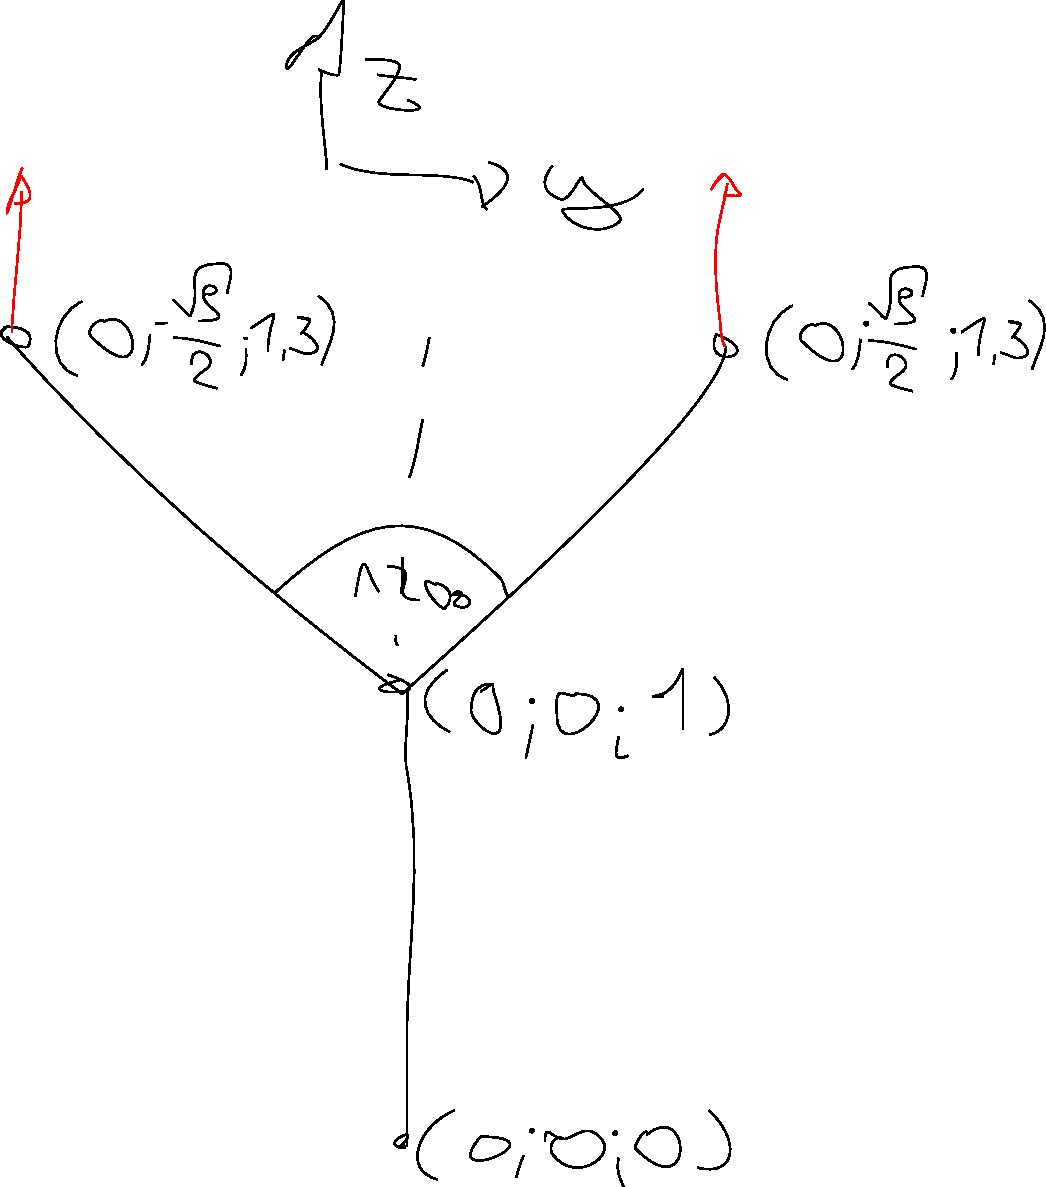
\includegraphics[scale=0.2]{pictures/example_3_lines}}


\subsubsection{inputfile:\protect \\
\protect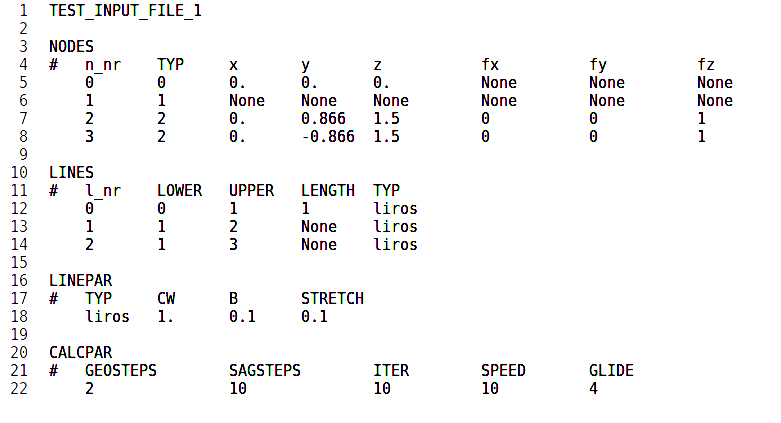
\includegraphics[scale=0.4]{pictures/input_3_lines}}


\subsubsection{matrix:\protect \\
\protect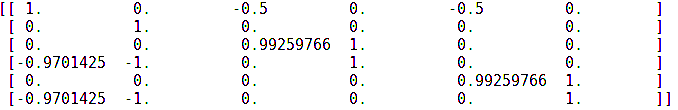
\includegraphics[scale=0.4]{pictures/matrix}}


\subsubsection{rhs:\protect \\
\protect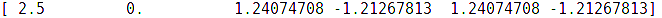
\includegraphics[scale=0.4]{pictures/rhs}}


\subsubsection{solution\protect \\
\protect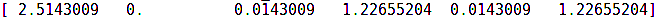
\includegraphics[scale=0.4]{pictures/solution}}


\subsubsection{visual output:\protect \\
\protect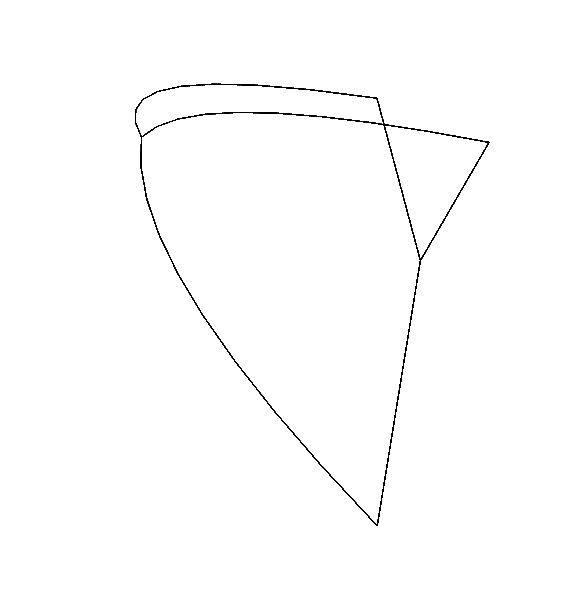
\includegraphics[scale=0.2]{pictures/visual_output}}

\newpage{}


\section{some functions}


\subsection{proj force}

\begin{align*}
(f_{l}\cdot\vec{l}).\vec{v}=f\\
f_{l}=\frac{f}{\vec{l}\cdot\vec{v}}
\end{align*}



\subsection{proj vec to surface:}

\begin{align*}
(\vec{p}+\vec{n}\cdot\lambda)=\vec{x}\\
\vec{n}.\vec{x}=\vec{n}.\vec{p}_{0}\\
\vec{n}.(\vec{p}+\vec{n}\cdot\lambda)=\vec{n}.\vec{p}_{0}\\
p_{0}=\begin{array}{c}
0\\
0\\
0
\end{array}\Longrightarrow\vec{n}.(\vec{p}+\vec{n}\cdot\lambda)=0\\
\vec{n}.\vec{p}=-(\vec{n}.\vec{n})\cdot\lambda\\
\lambda=\frac{-\vec{n}.\vec{p}}{\vec{n}.\vec{n}}
\end{align*}

\end{document}
